%!TEX root = ../main.tex
%Adding the above line, with the name of your base .tex file (in this case "thesis.tex") will allow you to compile the whole thesis even when working inside one of the chapter tex files
%: ----------------------- introduction file header -----------------------
\doublespacing
\chapter{Introduction}
\label{chap:intro}
Ancient passage tombs in Ireland show evidence that thousands of years ago, humans had an understanding of the movement of the Sun in the sky at different times of the year. These tombs are constructed such that only on the day of a solar solstice or equinox, is the passageway illuminated in full. Today the Sun is still a source of curiosity and has more than once shown that us humans are not the centre of the universe. The light and heat from the Sun are the essential source of energy for life on our planet however, our proximity to this star also comes with a risk. Explosive and energetic events such as coronal mass ejections and solar flares occur with varying frequency and intensity over the course of an eleven year cycle. Their effects on Earth were made known in a spectacular fashion in 1859 with the so called \textit{Carrington Event}. This was a solar eruptive event, the magnitude of which has not been seen in the subsequent 162 years. It induced currents into telegraph wires causing them to operate even though they had been removed from a power source. It also caused aurorae to be seen as close to the equator as Cuba and bright enough at higher latitudes that a newspaper could be read at night time under their light. 

The Sun emits across the electromagnetic spectrum, however the focus of this thesis is low frequency radio waves. Similar mechanisms that drive large energy releases like the Carrington Event also generate radio wave emission in the form of solar radio bursts. These solar radio bursts can be used as a remote diagnostic of the Sun's atmosphere and to determine physical processes in plasma in the outer layers of the solar atmosphere.
This chapter highlights some fundamental concepts of solar physics, different types of radio emission from the Sun and the implications of their study.

\section{The Sun}
The Sun is our nearest star and the centre of our solar system however, apart from these distinctions it is an average star. It is a G2 type star located on the main sequence of the Hertzsprung Russell diagram. It has a luminosity of $(3.83 \pm 0.04) \times 10^{26}$ W and a radius R$_\odot = (6.959 \pm 0.007) \times 10^8$ m \citep{Foukal2004}. The Sun's mass of $(1.9889 \pm 0.0003) \times 10^{30}$ kg comprises $>$ 99\% of the solar system's total mass \citep{Foukal2004}. At the time of writing, the Sun is $\sim$ 5 billion years old. Formed from a cooling cloud of gas and dust 4.6 billion years ago, the Sun now has a core with a temperature of 15 MK. This temperature is hot enough for nuclear fusion to occur and will continue to do so until the Sun's supply of hydrogen runs out. The Sun will remain on the main sequence for a further $\sim 5$ billion years before expanding into a Red Giant. %At this point the core will contract until the density reaches a density such that further condensation is prevented by the electron exclusion principle.   %There are a number of nuclear fusion processes in the Sun's core, the most common of which is the proton-proton or `pp' chain whereby four protons collide and fuse to form a Helium nucleus. The most frequent pp chain is known as ppI, it occurs 86\% of the time \citep{Turck-Chieze2011} and is as follows,
% $$
% ^1_1\mbox{H} + ^1_1\mbox{H} \rightarrow ^2_1\mbox{H} + e^+ + \nu_e
% $$
% $$
% ^2_1\mbox{H} + ^1_1\mbox{H} \rightarrow ^3_2\mbox{He} +\gamma
% $$
% $$
% ^3_2\mbox{He} + ^3_2\mbox{He} \rightarrow ^4_2\mbox{He} +2^1_1\mbox{H}
% $$
% Here, $^1_1\mbox{H}$ is a proton or hydrogen nucleus, $^2_1\mbox{H}$ is its isotope Deuterium, $^3_2\mbox{He}$ is the Helium isotope Triteum, $^4_2\mbox{He}$ is Helium, $e^+$ is a positron, $\nu_e$ is an electron neutrino and $\gamma$ is a gamma ray photon. A complete ppI chain releases $4.2 \times 10^{-12}$ J of energy in the form of electromagnetic radiation. The energy output of all pp chains account for 98.8\% of the total energy produced by the Sun \citep{Turck-Chieze2011}. 

% Photons generated in the ppI travel outwards from the core however, their small mean free path of 0.9cm means that this takes on the order of $10^5$ years to reach the solar surface \citep{Mitalas1992}. At 70\% of the Sun's radius (0.7 R$_{\odot}$), the temperature has cooled to 1 MK thereby allowing electrons to bind to atomic orbitals, drastically decreasing the scattering rate of photons. Energy transfer from here to the solar surface at 1 R$_{\odot}$ is now primarily done through convection. 
Due to our proximity to the Sun, we are able to observe a vast array of phenomena, many of which have direct terrestrial impacts. These phenomena take place in the solar atmosphere and shall be described briefly below. The study of these phenomena is a study of the plasma and magnetic field structure of the solar atmosphere and gives insights into energy generation and transport.
\subsection{The Photosphere}
The layer of the Sun at 1 R$_{\odot}$ is known as the photosphere and is what would be called the surface of the Sun. The temperature of the photosphere, alternatively the surface temperature of the Sun, is $\sim 6000$~K and has a number density of the order of $10^{17} \mbox{cm}^{-3}$, at which point the mean free path of visible photons becomes much greater than the distance between the Sun and the Earth and can be thought as coming directly from the solar surface.

The most distinct feature of the photosphere in white light are sunspots. Sunspots are seen as dark regions in the photosphere and are the manifestation of of solar activity. Sunspot magnetic fields are much stronger than the surrounding magnetic field of the photosphere and as such, inhibit heat transfer. This means that sunspots are cooler $\sim 4200$~K \citep{McLean1985} than the surrounding plasma.
%At this point, the mean free path of visible photons becomes much greater than the distance between the Sun and the Earth and can be thought as coming directly from the solar surface.
%This is the point at which the optical depth for visible light photons is 1 and their mean free path is much greater than the distance between scattering centres on the solar surface. 

Above the photosphere the temperature and density profile change dramatically, see Figure \ref{fig:corona_temp}, throughout the remaining layers of the Sun's atmosphere; the chromosphere, the transition region and the corona. 
\begin{figure}
    \centering
    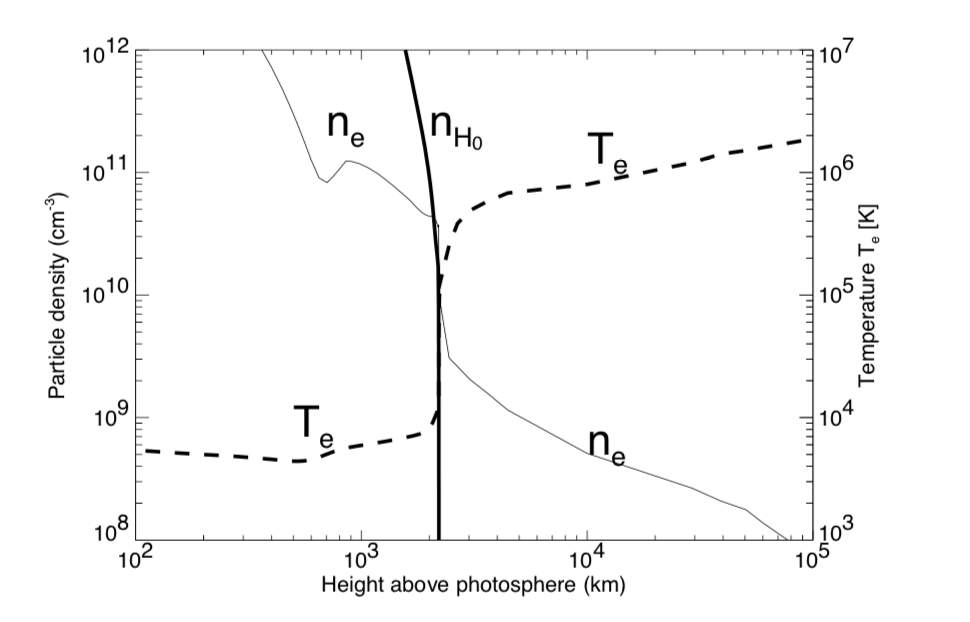
\includegraphics[width=\columnwidth]{Images/Corona_temp.png}
    \caption[Model of electron density and temperature with height in the solar atmosphere.]{Model of electron density and temperature with height in the solar atmosphere. The x axis shows height above the chromosphere in kilometres while the y axes show particle density in cm$^{-3}$ and temperature in Kelvin. The chromosphere begins $\sim 500$~km above the photosphere. The region around 2000 km showing a sharp rise in temperature and sharp fall in electron density is known as the transition region. Above this height plasma becomes fully ionised and is known as the corona. Image from \cite{Aschwanden2004}.}
    \label{fig:corona_temp}
\end{figure}
%Figure \ref{fig:Sun} shows the interior layers of the Sun and its atmosphere.
%\begin{figure}[t]
%    \centering
%    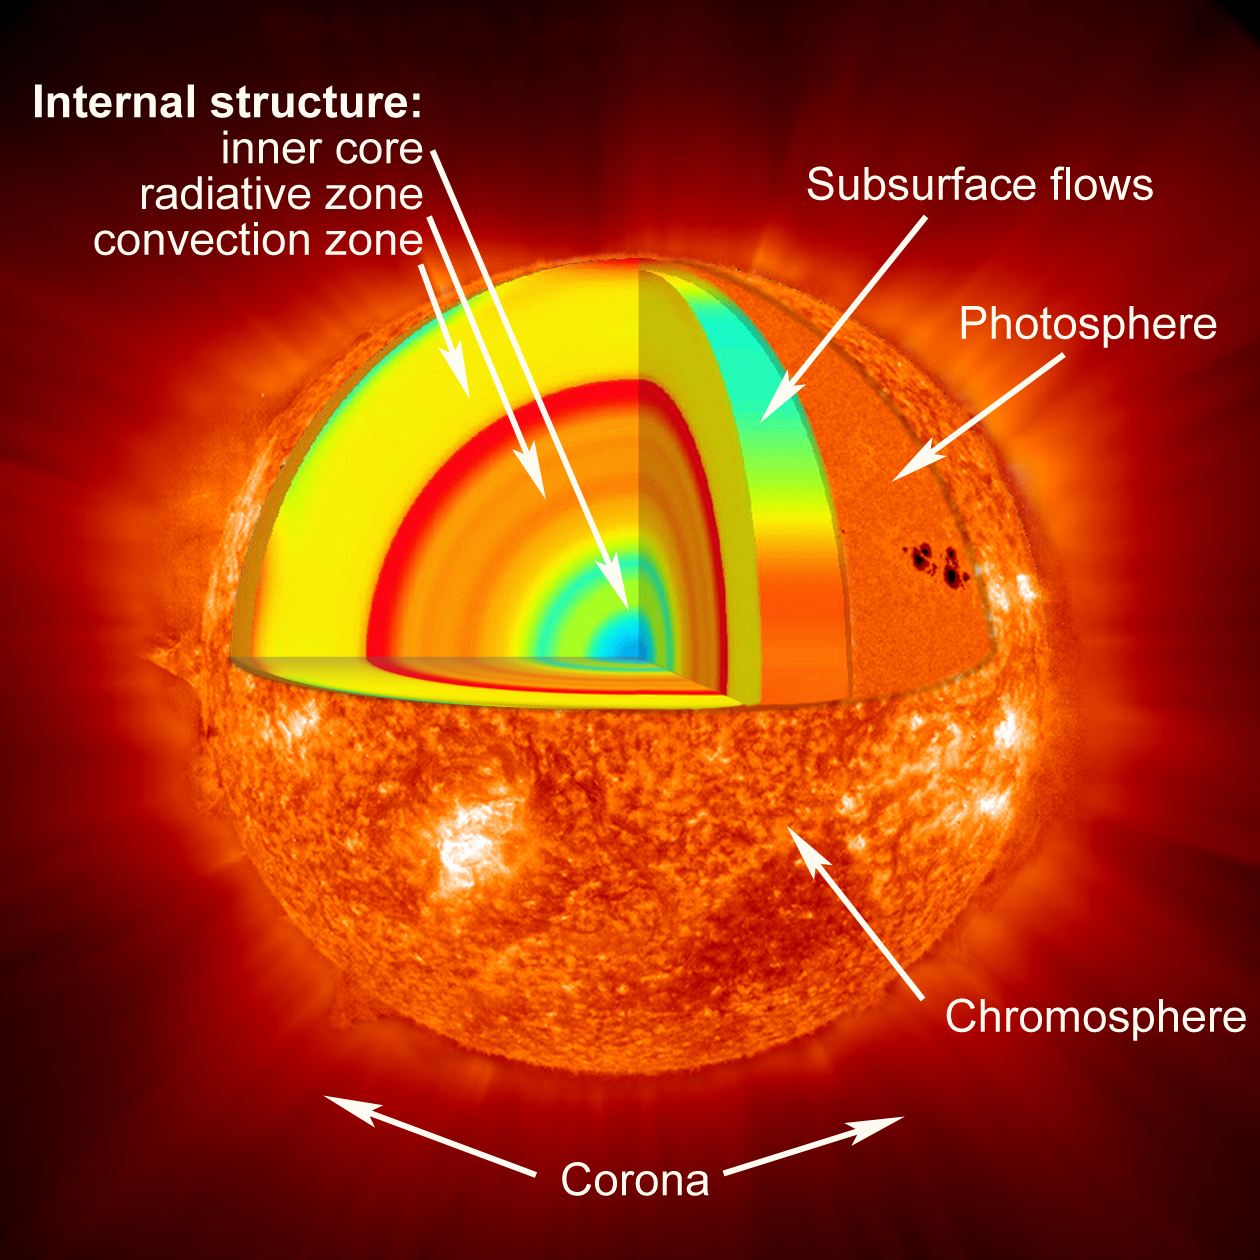
\includegraphics[width=0.5\columnwidth]{Images/Sun_interior.jpg}
%    \caption[Diagram of Sun's interior and atmospheric layers.]{Diagram of Sun's interior and atmospheric layers. Photons produced by nuclear fusion in the core transfer energy outwards through the radiative zone to ~0.7 R$_{\odot}$. At this point, convection becomes the main form of energy transport. The visible surface of the Sun is known as the photosphere and marks the boundary between the interior and the atmosphere. The solar atmosphere consists of three layers, the chromosphere, the transition region (not shown) and the corona.}
%    \label{fig:Sun}
%\end{figure}

\subsection{The Chromosphere}
In traditional plane-parallel models, the chromosphere extends to $\sim 2000$ km above the photosphere. Its name is derived from the Greek word for colour, $\chi \rho \omega \mu \alpha$ (\textit{chroma}), in reference to the red-coloured rim visible during solar eclipses. This red colour originates from the dominant hydrogen-$\alpha$ (H$\alpha$) transition at 656.3 nm. Temperatures in the chromosphere show a decrease with distance to a local minimum of $\sim 4400$ K at $\sim 500$ km above the photosphere. The temperature then rises again to a maximum of $\sim 20,000$ K at its upper boundary. These temperatures are low enough that most of the hydrogen in the chromosphere remains neutral. 

The chromosphere exhibits numerous structures and dynamics often observed in emission lines such as H$\alpha$, the Ca II H and K lines and the Lyman-$\alpha$ transition of hydrogen. The most prominent structural features of the quiet chromosphere include the chromospheric network on the disk and small, almost ubiquitous, jets of plasma known as spicules on the limb. The chromospheric network forms along the boundaries of supergranular cells where magnetic fields are concentrated. The magnetic field strength in the network can reach hundreds of millitesla although the average field strength of the chromosphere is $\sim 3$~mT \citep{McLean1985}.

% have been observed and are theorised to be a contributor to coronal temperatures.
% These are almost all due to the flux emergence of magnetic field in the chromosphere as evidenced by the supergranular structure. S

\subsection{The Transition Region}
The transition region occurs between the chromosphere and corona. Rather than a geometric layer, it is more accurate to consider the transition region as the region where the temperature rapidly increases (over distances as short as $\sim 100$ km) from $\sim 20,000$K to $\sim 0.8$ MK. Because the pressure remains approximately constant over this distance, the electron number density drops dramatically as is shown in Figure \ref{fig:corona_temp}. The transition region is also the part of the solar atmosphere where plasma changes from being partially ionised and collisionally dominated to fully ionised and collisionless. Network structures are also visible in low transition region images and are generally larger than those of the chromosphere, suggesting an expansion of magnetic flux tubes with height. However, the network completely disappears in higher altitude images hence, the magnetic field structure transitions from being ordered in the chromosphere to being extremely complex in the corona \citep{Tian2017}. Emission from the transition region is predominantly in the ultraviolet and extreme ultraviolet.

\subsection{The Corona}
The outermost layer of the solar atmosphere is called the corona. It contains hot, tenuous, inhomogeneous and time-varying plasma which extends from the top of the transition region into interplanetary space.
%which displays a number of interesting phenomena thought to be governed by its complex magnetic field. The corona begins $\sim 2500$ km above the photosphere after a layer in the Sun's atmosphere known as the transition region, where electron density decreases and temperature increases dramatically (Figure \ref{fig:corona_temp}). 
The electron density in the corona ranges from $10^{9} \mbox{ cm}^{-3}$ at the base to $10^{6} \mbox{ cm}^{-3}$ at distances of 1 R$_{\odot}$ from the solar surface. Densities vary throughout the corona. Sparse, underdense regions at the base of the corona known as coronal holes exhibit densities of $\sim ( 0.5 - 1.0) \times 10^8 \mbox{ cm}^{-3}$ whereas areas of high magnetic activity known as active regions have electron densities of $\sim 2 \times 10^9 \mbox{ cm}^{-3}$ \citep{Aschwanden2004}. Active regions are the coronal counterpart to sunspots and are best seen in EUV images of the Sun. The complex magnetic fields in active regions drive many of the solar phenomena such as solar flares and coronal mass ejections (CMEs).
 %Certain areas in the corona however, exhibit electron densities approximately an order of magnitude greater than the ``quiet Sun". Theses areas of high electron densities ar 

Observing the white light corona is done with a number of ground-based and space-based instruments called coronagraphs, that emulate the effect of a total eclipse. The Large Angle and Spectrometric Coronagraph \citep[LASCO;][]{Brueckner1995} on board the Solar and Heliospheric Observatory (SOHO) is one such instrument and allows the corona to be observed from distances of 2-32 R$_\odot$. The corona is also observed in extreme ultraviolet (EUV) lines, soft X-rays and at radio wavelengths. Observations at various wavelengths show a plethora of structure in the corona both on disk and on the limb that exist on varying time scales of a few minutes to a number of days. All particle acceleration events that produce radio emission of interest to this thesis occur in the solar corona. Figure \ref{fig:aia_quad} shows the corona and other layers of the solar atmosphere observed with the Atmospheric Imaging Assembly \citep[AIA;][]{Lemen2012}.

The sun observed at low radio frequencies looks different to that in EUV images, mostly due to the reduced spatial resolution of radio images. However, some key features of the solar corona are still seen in radio image, as depicted in Figure \ref{fig:qs_radio}. Here the contours show radio emission between 140 and 160~MHz and are overlaid on a 193{\AA} image taken with AIA. The peak in the contours is seen to overlap with a small active region while coronal holes show no radio emission.

The high temperature of the corona remains one of the greatest mysteries in all of solar physics. Energetic events in the corona such as solar flares and CMEs, described in \ref{subsec:sf} and \ref{subsec:CMEs}, are observed across the electromagnetic spectrum. They are studied in order to understand how particles are accelerated, how energy is released and ultimately, why the corona has such an unaccountably high temperature.

% have a diagnostic in radio spectra. This PhD focuses on studying these radio diagnostics at their highest temporal and spatial resolutions to date.
\begin{figure}
\centering
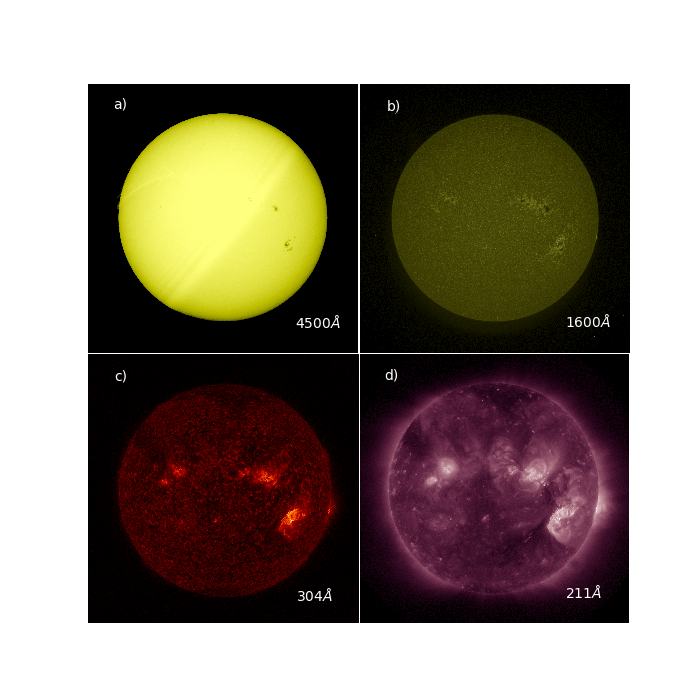
\includegraphics[width=0.8\columnwidth]{pm_aia_quad.png}
\caption[The solar atmosphere at different wavelengths.]{The Sun observed with AIA in four different wavelengths and thus in four different layers of its atmosphere. Panel a shows the photosphere at 4500{\AA}, a group of sunspots is visible towards the southwestern limb of the sun. Panel b shows the chromosphere at 1600{\AA} and exhibits the chromospheric network. Panel c shows the upper chromosphere and transition region at 304{\AA}. Panel d shows the upper corona at 211{\AA} the active region is noticeable as the bright region in the same location as the sunspot group as in panel a.}
\label{fig:aia_quad}
\end{figure}

\begin{figure}
\centering
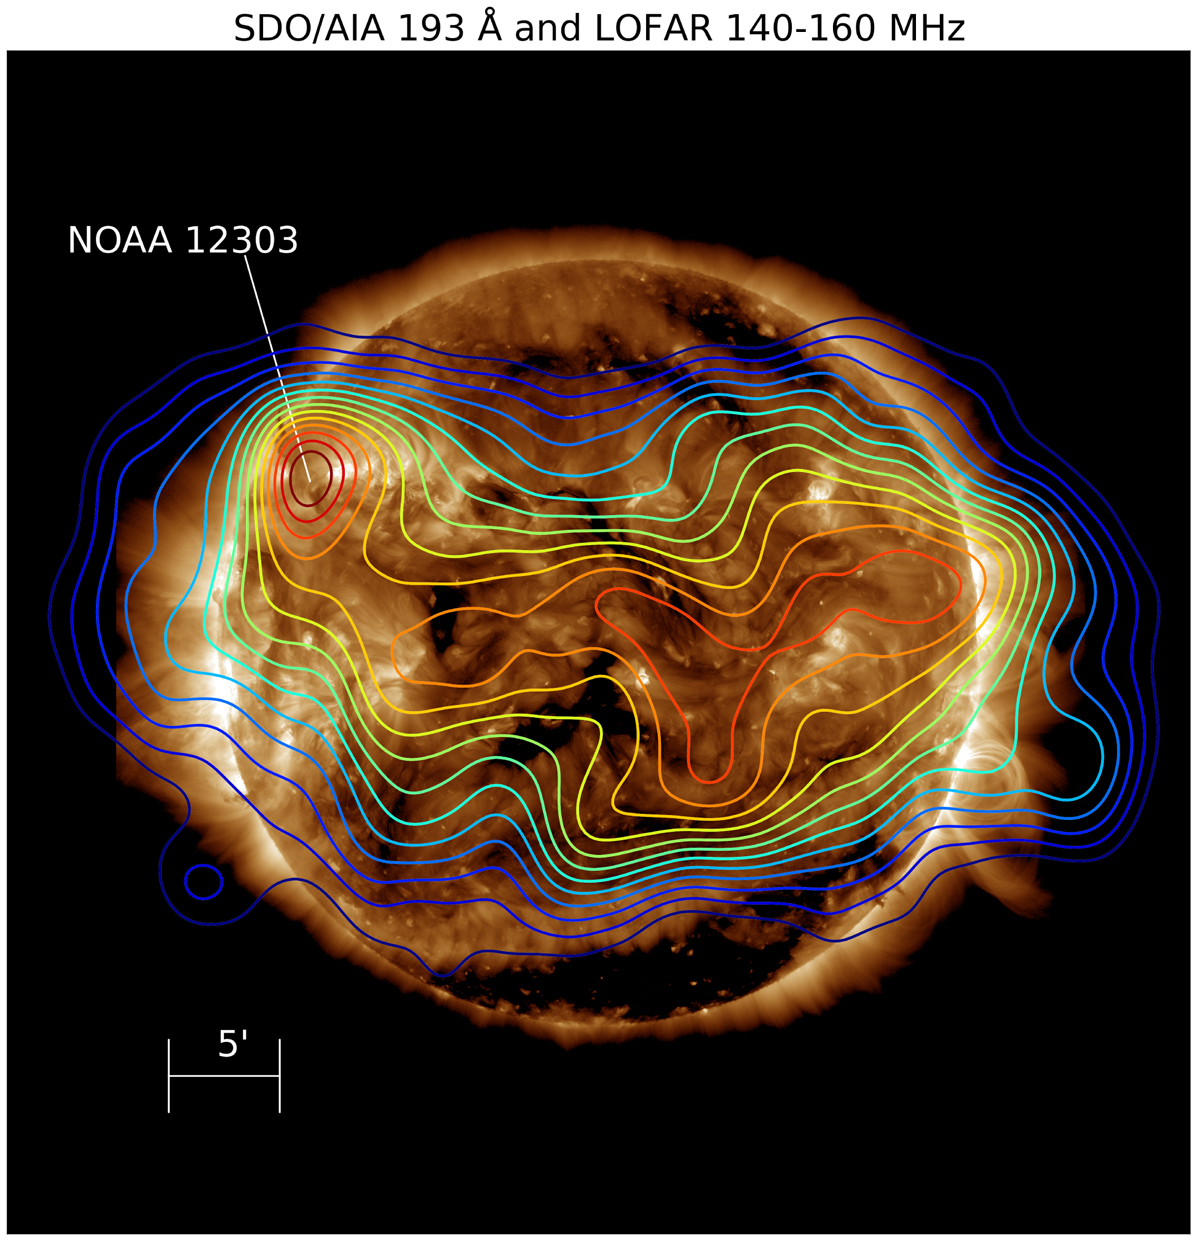
\includegraphics[width=\columnwidth]{Aoife_quiet_radio_sun.jpg}
\caption[The quiet Sun at low frequency radio wavelengths.]{The solar corona observed at low radio frequencies overlayed on a 193 {\AA} AIA image of the corona. The contours show the radio emission tracing out features in the solar corona, e.g. and intense peak above an active region and no emission around coronal holes. Image from \cite{Ryan2021}.}
\label{fig:qs_radio}
\end{figure}
\subsection{The Plasma Beta Parameter}
The plasma beta parameter is effectively a ratio of pressure due to the plasma and the magnetic field pressure. It is given, in SI units, as
\begin{equation}
\label{eq:pbeta}
\beta = \frac{nk_BT}{B^2/2\mu_0}
\end{equation}
where $n$ is the electron density, $k_B$ is the Boltzmann constant, $T$ is the plasma temperature, $B$ is the magnetic field strength and $\mu_0$ is the permeability of free space. Using values of $n$ and $T$ from Figure \ref{fig:corona_temp} and typical values for the magnetic field strength in the chromosphere ($\sim 100$~G) and corona ($\sim 10$~G) we can see that the value for $\beta$ changes from values $>1$ in the chromosphere to $<1$ in the corona. In low $\beta$ environments the magnetic pressure dominates and plasma is confined along magnetic field lines. It is for this reason that the magnetic field structure of the solar corona gives rise to a number of energetic phenomena such as solar flares and coronal mass ejections.
\section{Solar Flares}
\label{subsec:sf}
Solar flares are massive releases of magnetic energy commonly believed to be due to a reconfiguration in the complicated magnetic field structure in an active region.  They are some of the most energetic events in the solar system, releasing $\sim 10^{25}$ J of energy over a matter of minutes. Flares are observed across the electromagnetic spectrum from radio waves to $\gamma$ rays with energies $> 10$ MeV. They are classified by the amount of X-ray flux (W m$^{-2}$) detected by the Geostationary Operational Environmental Satellite (GOES) 1-8 {\AA} band on a logarithmic scale as being A, B, C, M or X class with A being the lowest flux ($10^{-8} \mbox{ W m}^{-2}$) and X the highest ($10^{-4} \mbox{ W m}^{-2}$). Each class is further subdivided into a linear scale.
A timeseries of X-ray flux from a solar flare is often called a lightcurve and has three characteristic phases; a pre-flare phase which shows X-ray flux associated with the active region where the flare occurs, an impulsive phase showing a sharp rise in X-ray flux corresponding to accelerated particles colliding with the solar surface, and a gradual decay phase where plasma heated by the flare gradually cools back to its pre-flare state. Figure \ref{fig:GOES_Xclass} shows a GOES light curve of the X9 class flare that occurred on 10 September 2017 and the three flare phases described above.

\begin{figure}
    \centering
    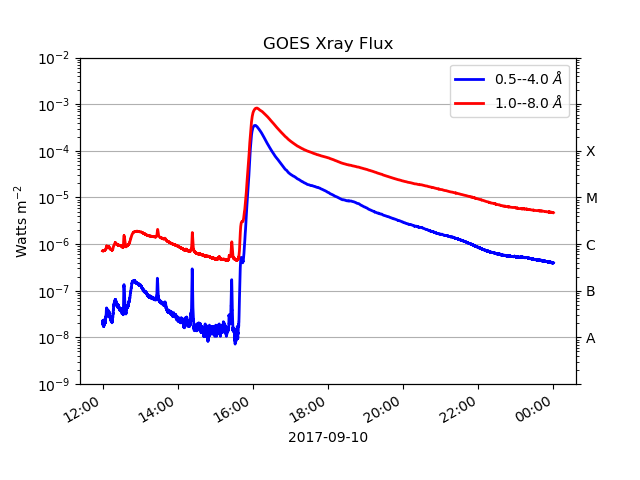
\includegraphics[width=\columnwidth]{Images/GOES_Xclass.png}
    \caption[GOES lightcurve for X9 class flare on 10 September 2017.]{The GOES lightcurve of the X9 flare that occurred on 10 September 2017. The x axis indicates the time of day on 10 September 2017 while the y axes show the X-ray flux in Wm$^{-2}$ and the flare classification. The red curve shows the 1-8 {\AA} channel by which the flare is classified while the blue curve shows the 0.5-4 {\AA} band. The three characteristic phases of a solar flare are clearly displayed here. The pre-flare phase before $\sim$ 16:00 UTC, the impulsive phase indicated by the sharp rise in flux and the gradual decay phase where X-ray flux gradually returns to the pre-flare level.}
    \label{fig:GOES_Xclass}
\end{figure}
During solar flares, magnetic structures known as coronal loops fill with hot plasma and begin to emit in soft X-rays. At the same time, electrons are accelerated towards the solar surface where their energy is converted to hard X-rays in the collision via bremsstrahlung. 

\section{Coronal Mass Ejections (CMEs)}
\label{subsec:CMEs}
In certain magnetic reconnection events, plasma suspended in a magnetic flux rope erupts from the corona into the heliosphere, the volume around the Sun where the interplanetary medium is dominated by particles flowing outward from the Sun. These eruption events are known as coronal mass ejections and accelerate 10$^{15}$ g of charged particles at typical speeds of up to $\sim 2500 \mbox{ km s}^{-1}$ \citep{Gopalswamy2000}. A ``textbook" CME structure consists of a bright front that surrounds a dark cavity and a bright central core. CMEs are observed using coronagraphs as they are much fainter than the solar disk. An example of a CME observed using the LASCO C2 corona with a field of view from 1.5 R$_\odot$ to 6 R$_\odot$ can be seen in Figure \ref{fig:CME}. Ejected material from a CME can interact with the Earth's magnetosphere and is known to have caused adverse effects including satellite communication disruption, radio blackouts, widespread power outages and large inaccuracies in GPS postions \citep{Eastwood2017}. CMEs can travel faster than the local Alfv\'{e}n speed in the corona leading to a shock which can accelerate particles. 

\begin{figure}
    \centering
    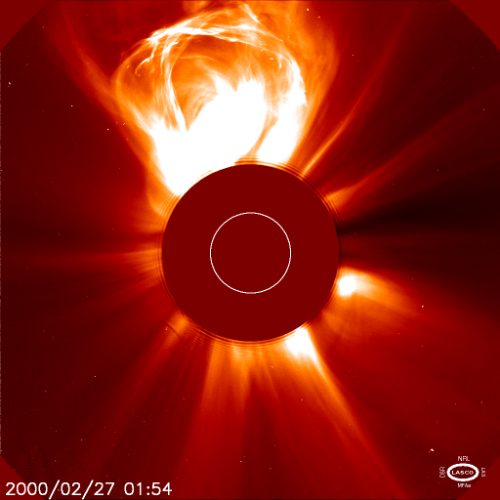
\includegraphics[width=0.75\columnwidth]{Images/LASCO_C2_CME.jpg}
    \caption[CME observed with the LASCO C2 coronagraph on 27 February 2000.]{A coronal mass ejection (CME) observed with the LASCO C2 coronagraph on 27 February 2000. The area covered by the coronagraph is shown in the red disk in the centre of the image and the white circle represents the solar disk. The bright feature in the top of the image is the CME while less bright structures known as streamers are also seen.}
    \label{fig:CME}
\end{figure}

\section{Solar Radio Bursts}
\label{sec:solar_radio_bursts}
In 1942 while Britain was monitoring radar signals for the signs of enemy aircraft, a strong, noise-like and highly variable signal was noticed by radar operators. Upon investigation it was found that this jamming was in fact radio emission from the Sun. The discovery of this radio emission being associated with a major solar flare was kept secret until after the war and was published by \cite{Appleton1946}.
Since then the field of solar radio astronomy has flourished and significant advancements in both instrumentation and theory have occurred. Worldwide, radio interferometers such as the LOw Frequency ARray \cite[LOFAR;][]{VanHaarlem2013} and the Murchison Widefield Array \citep[MWA;][]{Lonsdale2009} have been built while next generation interferometers like the Square Kilometre Array \citep[SKA;][]{McMullin2020} are slowly being brought online. These telescopes offer a dramatic improvement on the spectral resolution and imaging capability of those that were first used to study solar radio emission.

Solar radio emission often comes in the form of bursts of varying time scales. These were initially classified into three types by \cite{Wild1950b} with a fourth and fifth type being discovered by \cite{Boischot1957} and \cite{Wild1959} respectively. A wealth of other fine structure radio bursts are also observed, predominantly found in radio storms such as S bursts, drift pairs and stria \citep{McConnell1980,Melrose1982,NelsonandMelrose1985}. 
The fine structure of these bursts can often reveal information about small-scale turbulence in the corona \citep{Reid2021}.
Figure \ref{fig:burst_cartoon} shows a schematic of the five ``classic" types of solar radio burst. A brief description of some solar radio phenomena is given below.
\begin{figure}
    \centering
    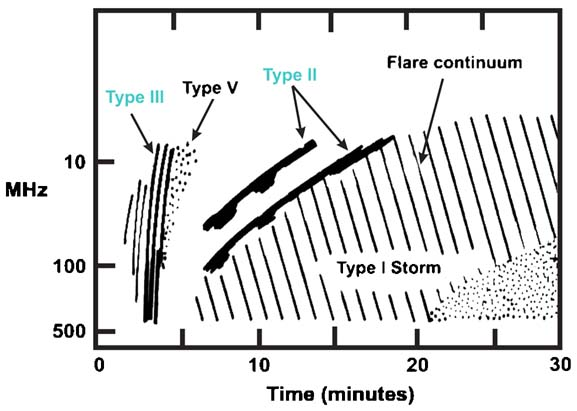
\includegraphics[width=0.75\columnwidth]{Images/Burst_cartoon.jpg}
    \caption[Cartoon of type I-V radio bursts.]{A cartoon of type I-V radio bursts. The x axis shows the time scale of the various bursts which can range from less than 1 minute to greater than 10 minutes. The y axis shows the typical frequency range of the bursts. The different drift rates of the different burst types are apparent. Image from \cite{Cliver2009}.}
    \label{fig:burst_cartoon}
\end{figure}
\paragraph{Type I bursts}
Type I emission can appear as bursts and/or a continuum originating from ``storm centres" that are associated with active regions. Type I storms can last for many days. Emission from type I bursts is highly circularly polarised in the o-mode (whereby light is circularly polarised in the opposite direction as electrons are gyrating about a magnetic field line) and is also particularly directional with an increase in intensity as active regions rotate to the centre of the disk. Unlike type II or III bursts, they do not exhibit a harmonic structure \citep{McLean1985}.
\paragraph{Type II bursts}
Type II radio bursts are a form of radio emission seen from the Sun and are identified by a slow ($\sim 0.1$~MHz~s$^{-1}$) drift to lower frequencies in dynamic spectra. The frequency drift can be used to find the velocity of the shock causing a burst if the electron number density as a function of height is known. The velocities of type II bursts are often found to be $\sim 1000 \mbox{ km s}^{-1}$, which is faster than the Alfv\'{e}n velocity in the quiet corona meaning a shock must be present \citep{NelsonandMelrose1985}. Other basic properties of type II bursts include:
\begin{enumerate}
    \item Narrow bandwidths of up to $\sim 100$~MHz from initial to final frequencies.
    \item A harmonic structure of two bands with a frequency ratio slightly less than 2:1 at a fundamental, $f_p$, and harmonic, $2f_p$, frequency can be seen for most type II bursts. This structure is consistent with the idea that type II emission is due to plasma oscillations.
    \item A large number of type II bursts contain band splitting into an upper and lower band for each of the harmonics in their spectra. The cause for this splitting is not fully understood but it is commonly thought that the two bands are related to emission upstream and downstream of the MHD shock front which causes the type II burst \citep{Smerd1974,NelsonandMelrose1985, Vrsnak2002}.
    \item Herringbone structure. Approximately 20\% of type II bursts show a herringbone structure of rapidly drifting emission spikes shooting out of the ``backbone" of the main frequency drift to higher and lower frequencies. These herringbones are thought to be due to electron beams being accelerated at the associated shock for the type II burst \citep{Mann1995}. While the backbone is poorly polarised, the herringbones have been found to be quite strongly ($\sim 70\%$) polarised. The level of polarisation of herringbones determined by \cite{Suzuki1980} are similar to those of type III bursts. They suggest that this is evidence that herringbone structure is due to plasma emission from accelerated electron beams such as in the case of type III bursts. 
    \item Starting emission frequencies of the order of a few 100~MHz ending at frequencies above 20~MHz. This being said, type II bursts with starting frequencies of $\sim 100$ kHz have also been observed. 
    These lower frequency bursts are thought to be due to interplanetary shocks whereas higher frequency bursts are considered to be from shocks in the low corona.
    \item Typical durations of 5-15 minutes. type II bursts that occur after a flare do so with a delay ranging from 2-20 minutes. Bursts with shorter durations generally have higher starting frequencies. %Timing and duration    
\end{enumerate}
 
Based on these and a number of other properties discussed in greater detail by \cite{NelsonandMelrose1985}, type II radio bursts can be used as indicators for MHD shocks in the solar corona. Observational proof of frequency varying inversely with time in the solar wind, consistent with radiation being generated at $f_p$ and $2f_p$ directly upstream from a CME-driven shock, was found by \cite{Reiner1997} and solidifies this argument.
\paragraph{Type III burst}
Observations of type III radio bursts (and their sub-categories) are of particular interest to this thesis and, as such, are described in Section \ref{sec:typeIII}.
\paragraph{Type IV burst}
Type IV bursts come in at least three sub-types with the general characteristic that they are of the from of broadband emission lasting for several hours. Early stationary type IV bursts (also known as the flare continuum) associated with the decay phase of solar flares, late stationary bursts which appear similar to type I emission, and moving type IV bursts which exhibit a smooth, wide-band spectrum \citep{McLean1985}.
\paragraph{Type V burst}
The last of the broadband emission bursts, type V radio bursts typically have a duration of 1-3 minutes and appear as an afterglow from type III bursts. Type V emission is strictly less than 150~MHz and is accepted that it results from electrons that generate a type III burst and become trapped in a closed magnetic loop in the corona \citep{McLean1985}.

\paragraph{Fine Structure: S bursts} 
S bursts, initially called Fast Drift Storm (FDS) bursts, were first observed at the Culgoora Solar Observatory in 1967 \citep{Ellis1969} They were later renamed by \cite{McConnell1980} who likened them to Jovian S bursts. They have a narrow bandwidth of the order of 0.03~MHz and a drift rate of 1-2~MHz~s$^{-1}$ and durations much less than 1s. \cite{McConnell1980} also concluded that S bursts are radiated at either the plasma frequency or its harmonic in a manner similar to type III bursts but that the implications of S burst fine structure and coronal scattering can only be defined once it is determined which harmonic of the plasma frequency they are radiated at. \cite{Melnik2010} propose a model of S bursts being generated by coalescence of fast magnetosonic waves with Langmuir waves which agrees well with the analysis of \cite{Clarke2019}. Modern observations of S bursts, such as those conducted using LOFAR's tied-array imaging mode \citep{Morosan2015}, can give greater insight into the spectral and temporal variability of S bursts and what this might mean for the environment they are generated in.
\\
\\The spatial extent and fine spectral structure of type III radio bursts are the main focus of this thesis. In Section \ref{sec:typeIII} below I outline the physical characteristics of type III bursts and their subcategories.

\subsection{Type III Bursts}
\label{sec:typeIII} 
Type III bursts are possibly the most useful radio burst for studying properties of plasma in the corona. As we shall see, they offer a remote measurement of the plasma density of the region where they are emitted. This allows us to probe the solar corona plasma using any of the many radio telescopes on Earth dedicated to solar radiophysics \citep[e.g.][]{Benz2004}.
\cite{Reid2014} review the observational properties of type III bursts which are repeated in brief here. The defining characteristic of type III bursts is a drift from high to low frequencies in a dynamic spectrum. The drift rates for type III bursts are typically quite fast, of the order of $\sim$ 10~MHz~s$^{-1}$ depending on the frequency. The frequency drift rate, $df/dt$, has been found to have various relations with frequency \citep{Reid2014} but most agree that $df/dt \propto f^{\alpha}$, where $\alpha$ ranges in the literature from $\sim 1$ to $\sim 2.7$. 

\cite{Ginzburg1958} proposed that type III bursts are emitted at the plasma frequency,
\begin{equation}\label{eq:1}
    \omega_{p}^2 = \frac{N_e e^2}{m_e \varepsilon_0}
\end{equation}
where $N_e$ is the number density of electrons, $m_e$ is the electron mass, $e$ is the electron charge and $\varepsilon_0$ is the permittivity of free space. A more detailed description of the plasma emission process is given in Section \ref{sec:plasma_emission}.
Although Eq. \ref{eq:1} is relatively simple, it contains an important relationship in plasma physics. Namely, the plasma frequency is proportional to the square root of the electron density. This means that plasmas at higher electron densities will oscillate at higher frequencies than those of lower densities. The drift in type III bursts, which are emitted at $\omega_p$, is therefore an indication of the emission source moving from an area of high electron density to low density, i.e. from the lower to the upper corona. Using a model of electron density in the corona such as the \cite{Newkirk1961} model, it can be inferred that the exciter of type III bursts has a speed of $\sim 0.3$~c.

\begin{figure}
    \centering
    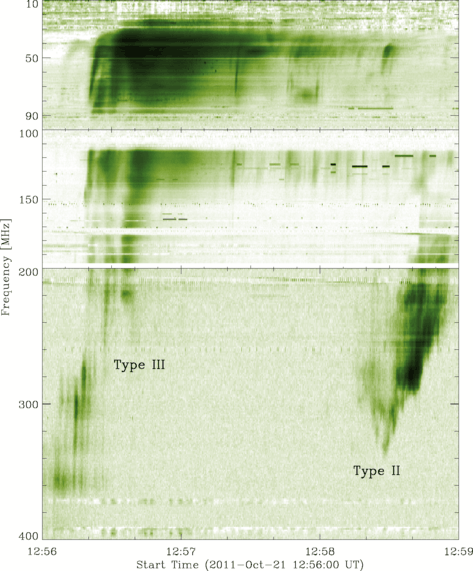
\includegraphics[width=0.75\columnwidth]{Images/Pietro_typeIII.png}
    \caption[A number of type III bursts observed by \cite{Zucca2012} on 21 October 2011.]{A number of type III bursts observed by \cite{Zucca2012} on 21 October 2011. The x axis gives the time on 21 October 2011 while the y axis shows the frequency in MHz. A number of type III bursts extend to frequencies below 200~MHz. A type II burst can be seen between 140 and 330~MHz later in the day.}
    \label{fig:bursts}
\end{figure}

Type III bursts are observed to be in two bands, a fundamental and harmonic band that are emitted at $\omega_p$ and $2 \omega_p$ respectively. Both bands exhibit the same frequency drift although the flux of the harmonic band is usually less than that of the fundamental band \citep{Wild1954a, McLean1985}. The process of plasma emitting radio frequencies at $\omega_p$ and $2 \omega_p$ will be explained in more detail in Chapter \ref{chap:theory}. 
Figure \ref{fig:bursts} shows type III radio bursts below 400~MHz observed by \cite{Zucca2012}. A type II burst was also observed between 140 and 330~MHz and exhibits a much slower frequency drift than the type III bursts. A type III storm can be seen below 200~MHz. This is when type III emission is continuous over the span of large time scales and can last days. Type III bursts come in a number of subcategories described below.

\paragraph{Reverse and bi-directional bursts.}

A typical type III burst is produced when an electron beam travels along a magnetic field line away from the Sun to areas of lower density. If, instead, electrons travel towards the Sun to areas of higher density a reversed frequency drift is observed. Bursts where both the regular and reverse drifts can be seen simultaneously are bi-directional bursts \citep{Reid2014}.

\paragraph{Type IIIb bursts.}

\begin{figure}
\centering
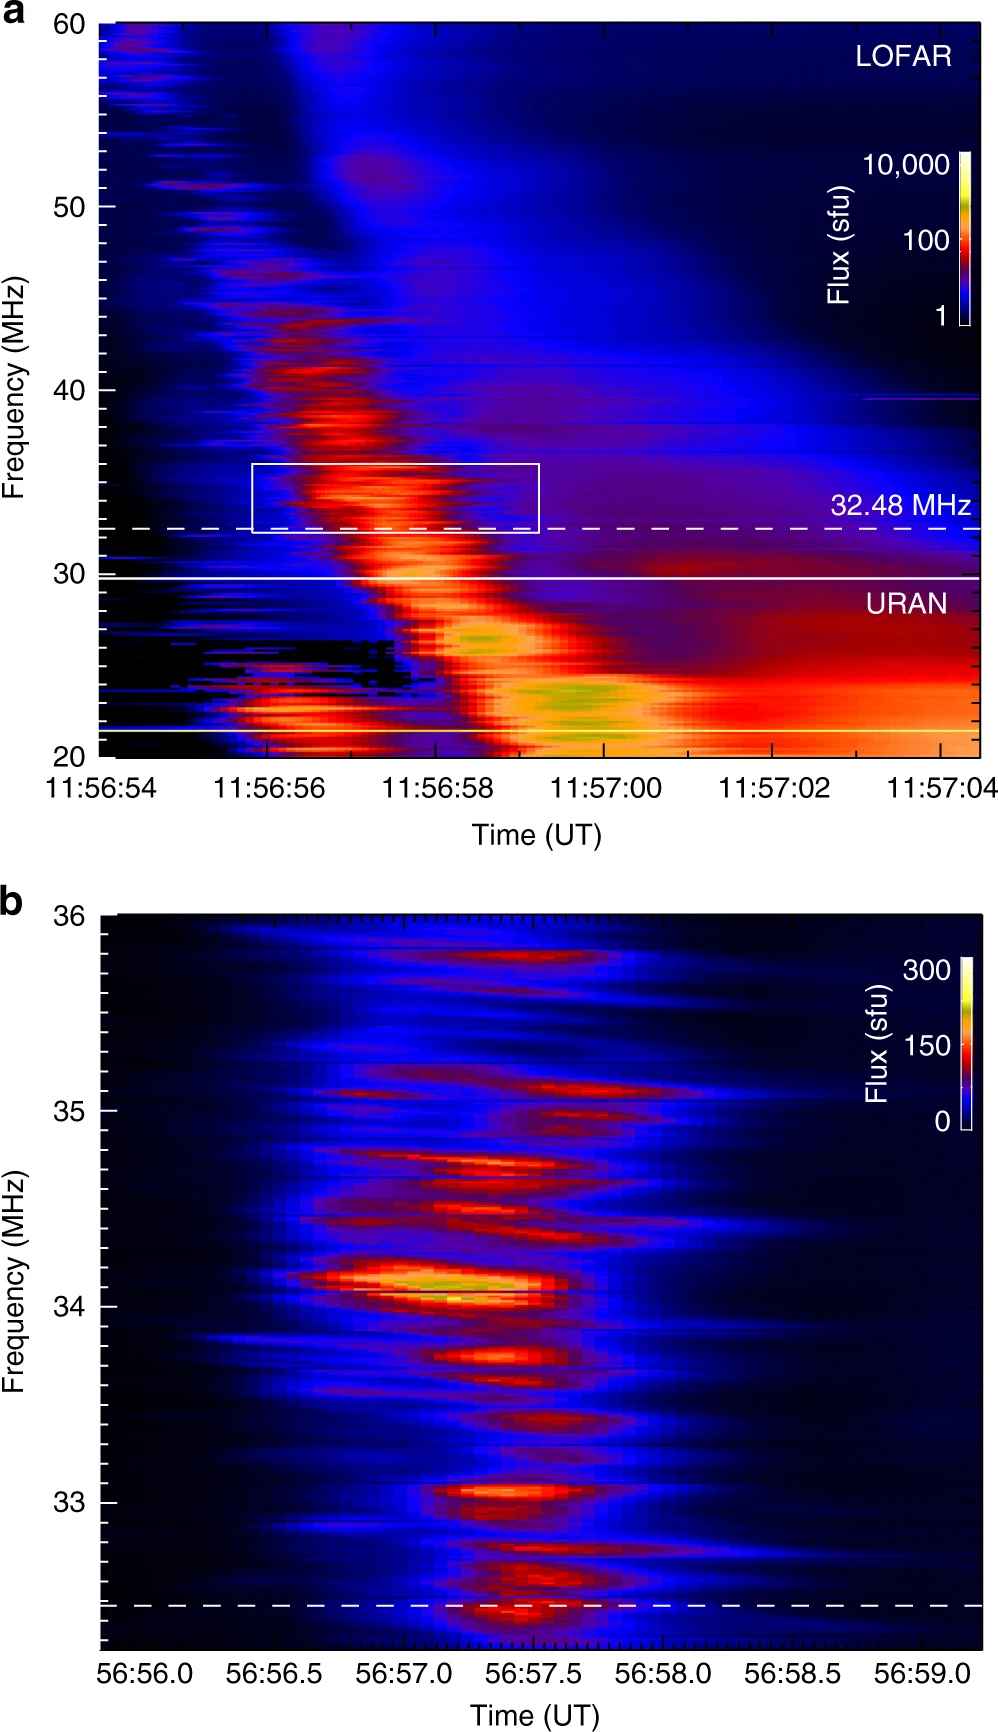
\includegraphics[width=0.5\columnwidth]{typeIIIbKontar.png}
\caption[The type IIIb radio burst from \cite{Kontar2017}.]{A type IIIb radio burst on 16 April 2015 analysed by \cite{Kontar2017}. Here the x axes show the time and the y axes show frequency in MHz. The colourbars denote the flux of the radio burst measured in solar flux units (1 sfu = $10^4$ Jy). Panel a shows the full duration of the type IIIb. Panel b is a zoom in of the 3 second wide box in panel a.}
\label{fig:typeIIIbKontar}
\end{figure}

Fine frequency structures are sometimes seen in type III bursts. Type IIIb radio bursts are defined as a number of narrow, nearly horizontal, frequency bands called striae, or striations, in the envelope of a type III. The frequency width of an individual striae is typically 0.05~MHz \citep{McLean1985} and they have a frequency drift rate of $\lesssim 150$~kHz~s$^{-1}$, which implies a speed of 0.6~Mm~s$^{-1}$ \cite{Sharykin2018}. Figure \ref{fig:typeIIIbKontar} shows a dynamic spectrum of a type IIIb burst from \cite{Kontar2017}. Individual striae can be clearly seen in panel b of Figure \ref{fig:typeIIIbKontar}. The theory describing the origin of this fine frequency structure has recently been revisited by \cite{Reid2021} who found that the striations are due to turbulence in the corona and their drift a result of moving Langmuir waves.

\paragraph{Type U and J bursts.}

In the case where electrons are travelling along a closed magnetic field line, a turning point in the frequency drift of a type III burst can be observed. For electrons that generate radio emission down to the footpoint of the magnetic field line, a U burst is observed. A U burst can be identified as an inverted U on a dynamic spectrum. More often, electrons stop generating radio emission as they travel back down the magnetic field line so only the turning point in frequency drift is visible in dynamic spectra. These are known as J type bursts. U and J bursts are far less common than type III bursts, despite the similar number of open and closed magnetic field lines along which electron beams can propagate. The reason for this proposed by \cite{Reid2017} is that the length of these closed loops is not long enough for the electron beam to become unstable to Langmuir waves.

\paragraph*{} The study of type III bursts offers an insight into the process of Langmuir wave generation in the solar corona and as such are an important tool in understanding the physics of coronal plasma \citep{Reid2014}. However, the effects of radio wave propagation from the source to the observer through the corona must but understood before inferences can be drawn from observations. 

\subsection{Low Frequency Radio Wave Scattering}

Spectral analysis of short temporal radio bursts with small bandwidths at $\sim 30$~MHz suggests that source sizes in the corona are of the order $\lesssim 1$ arcmin \citep{McConnell1980, Kontar2017}. Radio images of the Sun at metric and decametric wavelengths have yet to reveal this level of spatial structure. This was mostly due to the limitations of angular resolution of radio telescopes at the time. 
Observations with modern interferometers at these frequencies however, still have not observed spatial structure at these scales. The suggestion that there is a fundamental limit imposed upon the level of resolution obtainable by scattering of radio waves in a turbulent corona \citep{Bastian1994} has re-emerged in recent years \citep{Thejappa2007,Thejappa2008,Kontar2017,Kontar2019}. 

The development of scattering theory stems from \cite{Chandrasekhar1952} description of light scattered by a thin screen and will be outlined further in Chapter \ref{chap:theory}. The implementation of this theory into computational modelling has also seen considerable development since the first ray tracing experiments by \cite{Fokker1965}. \cite{Steinberg1971} built upon this by including the effect of spherical refraction through the corona and were able to obtain the time response of a scattered pulse source.

Both \cite{Fokker1965} and \cite{Steinberg1971} followed from \cite{Chandrasekhar1952} and assumed density inhomogeneities in the corona had a Gaussian power spectrum. However, it is now known that this assumption is incorrect. \cite{Bastian1994} provides a review of the work by \cite{Coles1989} and others to determine the shape of density inhomogeneity power spectrum. At large scales, greater than a few hundred kilometres, the spectrum is well described with a power law index of -5/3, which agrees with the Kolmogorov description of turbulence \citep{Kolmogorov1941} of density fluctuations with respect to size scale. For scales smaller than these but greater than a few kilometres, the spectrum becomes shallower and is better described with a power law index of $\sim 3$. Finally, on the smallest scales less than a few kilometres the spectrum steepens again. This steepening has been interpreted as the scale at which energy is dissipated by turbulence. \cite{Coles1989} also found that this inner scale increases with heliocentric distance. \cite{Bastian1994} expanded on this description of the density inhomogeneity power spectrum and investigated the angular broadening of radio waves sources at centimetre wavelengths.

The latest development in the modelling of radio wave scattering is by \cite{Kontar2019}. Rather than using the small scattering angle approximation of previous work, \cite{Kontar2019} build on the work of \cite{Arzner1999} and \cite{Bian2019}. In this approach, the effect of anisotropic density inhomogeneities is treated as photon diffusion in momentum space and the Hamiltonian equations for photon position and momentum can be solved iteratively to trace a photon's path. This allows for a continuous transition from weak to strong scattering, whereas previous work is limited to regime of small angle scattering. 

Understanding radio wave propagation effects, in particular scattering, is important because they affect all observations made at radio wavelengths. Radio wave scattering has been shown to depend on the relative level of density fluctuations in the corona and as such, offers a chance to learn about its turbulent nature. By classifying the power spectral density of these fluctuations it may be possible to gain an understanding of the turbulent processes that transport energy to the microscopic scales and result in the heating of the corona. 

\section{Thesis Outline}
The high spatial, temporal and spectral resolution of modern radio interferometers such as LOFAR and the launch of new space missions including Parker Solar Probe \citep[PSP;][]{Fox2016} and Solar Orbiter \citep{Muller2020} has ushered in a new age of solar radio observations. By developing a computational backend and using a unique method for fitting interferometric visibilities, this thesis has furthered the capability of an international LOFAR station and extracted value from existing interferometric observations. This thesis outlines how such developments have improved our knowledge of radio wave propagation in the solar corona using observations at some of the highest spatial, spectral and temporal resolutions available. In Chapter \ref{chap:theory} I outline the relevant background theory for the work presented in this thesis. Chapter \ref{chap:instrumentation} will describe the instrumentation used throughout this thesis, namely LOFAR, and the mathematical background for interferometric imagining. 

The REALtime Transient Acquistion backend (REALTA), is a seven node computer cluster designed to record and analyse the raw beamformed data from international LOFAR stations in real-time. The development of REALTA for solar and a myriad of other observations formed a key part of this work. Chapter \ref{chap:REALTA} describes the hardware and software of REALTA and showcases some first light observations.
 
The study of radio wave scattering in the solar corona has undergone a renaissance in recent years both in terms of computational modelling and observations. Chapter \ref{chap:measuring_source_sizes} will describe how, for the first time, LOFAR visibilities were fitted directly to determine the size and position of a type IIIb burst. This lead to a more subtle understanding of the root mean squared fluctuations of electron density in the solar corona, the key parameter necessary to quantify the effect of scattering. 

In order to accurately compare between models of the solar corona, in Chapter \ref{chap:observations_vs_theory} I present 29 type III radio bursts and determine their size and position using the visibility fitting technique with a Markov Chain Monte Carlo optimization. The results of this show that type III bursts exhibit an intrinsic source size greater than the size of a point source that has been scattered and highlights discrepancies between observations and computational modelling.

Chapter \ref{chap:future} includes a discussion on the future work that can be carried out from the foundations of this thesis. It outlines the necessary further studies needed to further our knowledge of radio wave scattering and how to utilise even higher temporal resolution observations of the radio sun. Chapter \ref{chap:future} will also contain a summary and conclusion of the work presented in this thesis.

